\documentclass[11pt]{article}
% Time-stamp: <homework-02.tex, saved on Fri, Sep 14, 2007 at 12:46pm>
\usepackage[margin=1in, head=1in]{geometry}
\usepackage{amsmath, amssymb, amsthm}
\usepackage{fancyhdr}
\usepackage{graphicx}
\usepackage{pgfplots}

%\usepackage{pdfsync}
\addtolength{\textwidth}{.5in}
\addtolength{\leftmargin}{-1in}
\addtolength{\textheight}{.5in}
\addtolength{\topmargin}{-0.5in}

%\pagestyle{fancy}
%\lhead{MATH 200X }
%\chead{Fall 2007}
%\rhead{FINAL EXAM}
%\lfoot{}
%\cfoot{\thepage}
%\rfoot{}

\setcounter{secnumdepth}{0}
%\renewcommand{\theenumi}{\alph{enumi}}
%\renewcommand{\emptyset}{\varnothing}
\newcommand{\R}{\mathbb{R}}
\newcommand{\N}{\mathbb{N}}
\newcommand{\Z}{\mathbb{Z}}
\newcommand{\clm}{\par\textit{Claim:}\par}
\newcommand{\diam}{\mathrm{diam}}
\newcommand{\sect}{\textsection}

\parindent=0in
\parskip=0.5\baselineskip

\begin{document} 

\begin{center}MATH 156: Precalculus  \\ Fall 2015 \\ Worksheet \sect 2.6: Transformations of Graphs\end{center}

\hrulefill

By the end of this section, you want to  know the transformations below affect the graph of $f(x).$ (Assume $c>0.$)
\begin{itemize}
\item $f(x+c)$ [translates $c$ units left]
\item $f(x-c)$ [translates $c$ units right]
\item $f(x)+c$ [translates $c$ units up]
\item $f(x)-c$ [translates $c$ units down]
\item $-f(x)$ [reflects about the $x$-axis]
\item $f(-x)$ [reflects about the $y$-axis]
\item $cf(x)$ [stretches or shrinks vertically]
\item $f(cx)$ [stretches of shrinks horizontally]
\item $|f(x)|$ [reflects portions of the graph below the $x$-axis to be above the$x$-axis]
\end{itemize}

\hrulefill

Example: Graph $f(x)=\sqrt{x},$ $g(x)=\sqrt{-x},$ $h(x)=-\sqrt{x}.$ Plot at least three points on each graph to confirm you picture is correct.\\

\newpage

Below is graphed the function $h(x)=x(x-2)(x+2)=x^3-4x$ and the line $y=4.$ Use the graphs to answer questions (a) through (e).

\begin{tikzpicture}[baseline=(current bounding box.center), xscale=1.5, yscale=.3]
\draw[<->] (0,-15) -- (0,15) node[above] {$y$};
\draw[<->](-3,0) -- (4, 0) node[right] {$x$};
\foreach \i in {-2,-1, 1, 2,3, 4,}{\draw (\i, .1) -- (\i, -.1);
\draw (\i,0) node[below] {\i};
}
\foreach \i in {-10,-5,5,10}{
\draw (-.1, \i) -- (.1,\i);
\draw (0,\i) node[  left] {\i};
}
\draw[smooth,samples=200,domain=-3:3, ultra thick,,<->]  plot({\x},{\x^3-4*\x)});
\end{tikzpicture}

On the graphs below, sketch (i) $y=3(x^3-4x)$, (ii) $y=(-1/2)(x^3-4x)$, (iii) $y=\vert x^3-4x \vert$\\
(i)
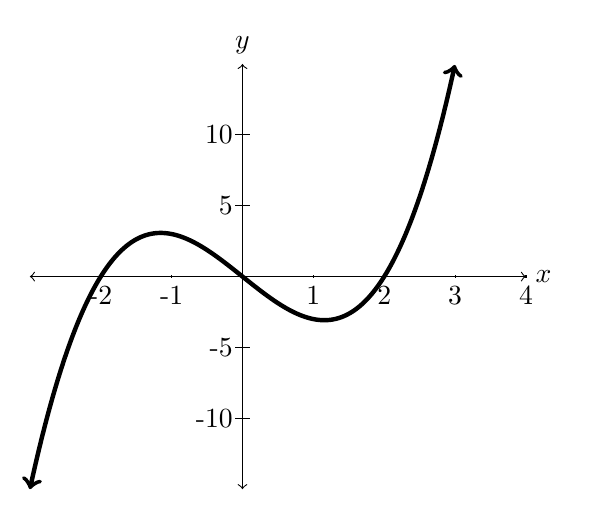
\begin{tikzpicture}[baseline=(current bounding box.center), xscale=.9, yscale=.18]
\draw[<->] (0,-15) -- (0,15) node[above] {$y$};
\draw[<->](-3,0) -- (4, 0) node[right] {$x$};
\foreach \i in {-2,-1, 1, 2,3, 4,}{\draw (\i, .1) -- (\i, -.1);
\draw (\i,0) node[below] {\i};
}
\foreach \i in {-10,-5,5,10}{
\draw (-.1, \i) -- (.1,\i);
\draw (0,\i) node[  left] {\i};
}
\draw[smooth,samples=200,domain=-3:3, ultra thick,,<->]  plot({\x},{\x^3-4*\x)});
\end{tikzpicture}
(ii) 
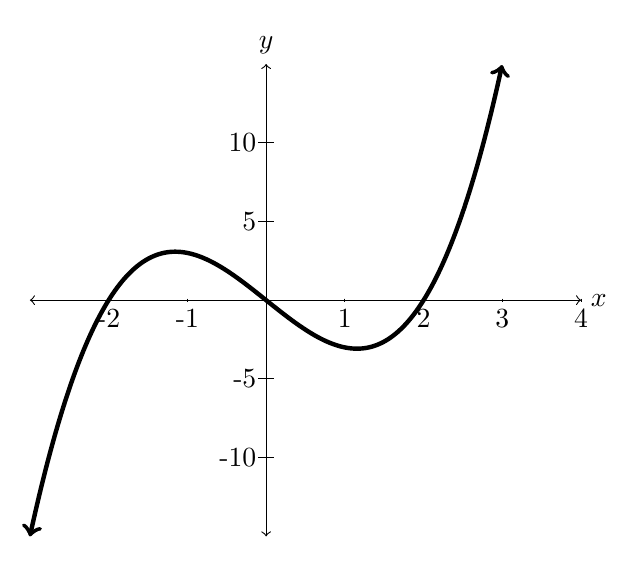
\begin{tikzpicture}[baseline=(current bounding box.center), xscale=1, yscale=.2]
\draw[<->] (0,-15) -- (0,15) node[above] {$y$};
\draw[<->](-3,0) -- (4, 0) node[right] {$x$};
\foreach \i in {-2,-1, 1, 2,3, 4,}{\draw (\i, .1) -- (\i, -.1);
\draw (\i,0) node[below] {\i};
}
\foreach \i in {-10,-5,5,10}{
\draw (-.1, \i) -- (.1,\i);
\draw (0,\i) node[  left] {\i};
}
\draw[smooth,samples=200,domain=-3:3, ultra thick,,<->]  plot({\x},{\x^3-4*\x)});
\end{tikzpicture}
\\ 

(iii)
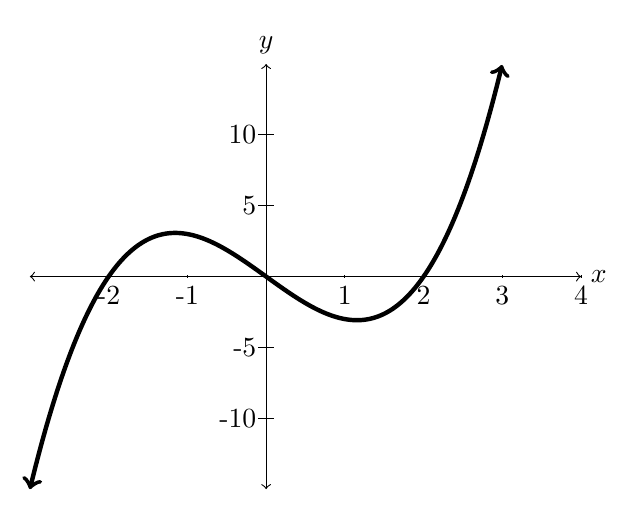
\begin{tikzpicture}[baseline=(current bounding box.center), xscale=1, yscale=.18]
\draw[<->] (0,-15) -- (0,15) node[above] {$y$};
\draw[<->](-3,0) -- (4, 0) node[right] {$x$};
\foreach \i in {-2,-1, 1, 2,3, 4,}{\draw (\i, .1) -- (\i, -.1);
\draw (\i,0) node[below] {\i};
}
\foreach \i in {-10,-5,5,10}{
\draw (-.1, \i) -- (.1,\i);
\draw (0,\i) node[  left] {\i};
}
\draw[smooth,samples=200,domain=-3:3, ultra thick,,<->]  plot({\x},{\x^3-4*\x)});
\end{tikzpicture}

\newpage

On the same axes, graph $f(x)=x^2+1,$ $g(x)=(3x)^2+1,$ and $h(x)=\left(\frac{x}{2}\right)^2+1$
\vfill

Graph $f(x)=\frac{-1}{x-2}+3$\\
\vfill
Graph an even function and an odd function.
\vfill


\end{document}

